\chapter{Aplicações}\label{ch:apl}

Neste Capítulo serão descritos os modelos das atividades aplicadas. As atividades foram divididas em dois tipos principais: Oficinas de Resolução de Problemas (ORP) e Atividades de Sala de Aula (ASA). No Capítulo \ref{ch:resanddisc} serão detalhadas algumas particularidades de cada aplicação, bem como os resultados e observações obtidos, dando continuidade às informações contidas no presente capítulo.

Na Seção \ref{sec:orp} são descritas as origens das ORP, a partir do contexto social em que estávamos inseridos, e suas modificações. Foram realizadas três oficinas ao todo, sendo que houve a necessidade de um \textit{redesign} para sua continuidade.

Na Seção \ref{sec:asa} estão descritas as ASA, as quais tiveram, assim como as ORP, três aplicações. As Atividades de Sala de Aula surgiram de um \textit{redesign} a partir de necessidades surgidas dos desdobramentos encontrados nas ORP.

\section{Oficinas de Resolução de Problemas} \label{sec:orp}

A Figura \ref{fig:ativEvo} mostra a evolução das atividades aplicadas ao longo deste trabalho. De forma sucinta, a ORP 1, representada em Azul passa por um processo de \textit{redesign} (em Verde) gerando um novo padrão de ORP. 

Esse novo padrão é representado pelas ORP 2 e ORP 3 (em Verde). Os resultados obtidos por estas ORP favoreceram a formação de um novo \textit{redesign}, representado em Laranja. Esse \textit{redesign} aplicado às duas ORP da origem às ASA.

\begin{figure}[htp]
\begin{center}
\caption{Evolução das atividades}
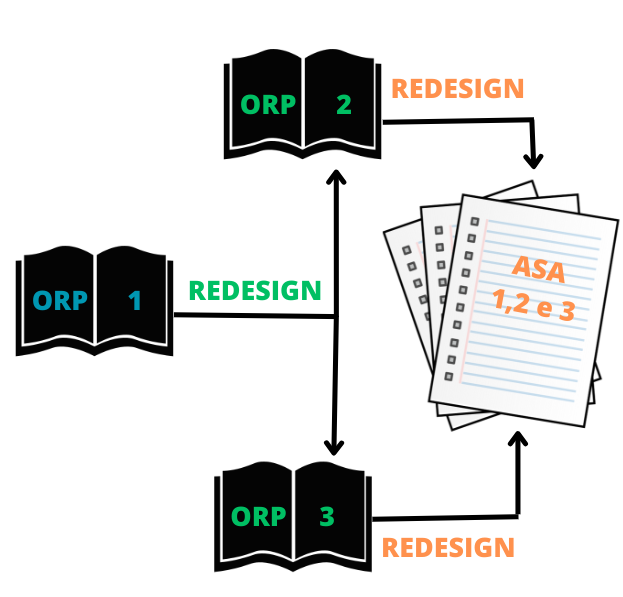
\includegraphics[width=0.9\textwidth]{fig/resumoatovodades.png}
\label{fig:ativEvo}
\caption*{Fonte: Criação do Autor.}
\end{center}
\end{figure}

Dessa forma, aplicamos os conceitos do EDR (a partir do \textit{redesign}), dentro dos modelos de aplicação da RP. E esses modelos estão baseados na metodologia de \textit{Scaffolding}. Assim, conseguimos perceber a conexão do tripé \textit{Scaffolding}, RP e EDR.

O processo de desenvolvimento desta dissertação iniciou no final do ano de 2019, com a redação do pré-projeto de pesquisa feito para o ingresso no programa de pós-graduação (que ocorreu no primeiro semestre de 2020). A proposta inicial era de fazer uma aplicação computacional (SBC). Nessa proposta o aluno receberia uma questão por vez, tendo a opção de solicitar uma dica, caso necessitasse. O próprio software forneceria opções de dicas para o aluno que escolheria uma opção mais próxima de sua necessidade.

Para cada questão seria atribuída uma pontuação. Essa pontuação teria seu valor máximo reduzido, à medida que o aluno fosse fazendo uso das dicas disponíveis. Neste Capítulo traremos uma análise sobre as observações obtidas ao longo das três oficinas de resolução de problemas. Para isso, escrevemos três Seções, uma para cada oficina. Relembrando, intitulamos como Primeira Oficina àquela aplicada a uma turma de Física Básica logo no início do período da pandemia.  

A Segunda Oficina foi aplicada também a uma turma de Física Básica, porém já havendo retornado as aulas presenciais. Por fim, a Terceira Oficina foi aplicada, ao mesmo tempo da Segunda Oficina, mas em uma turma de Física Avançada. 

Como já foi explicado, na Seção anterior, o funcionamento individual de cada oficina, aqui trataremos das observações e impressões de cada uma. Além disso, traremos algumas informações adicionais que possam ser de interesse. 

A função do \textit{Scaffolding} é manter o aluno trabalhando, sem que ele desista da questão. De forma com que o aluno consiga fazer o seu melhor durante o processo de resolução, mesmo que para isso acabe obtendo uma pontuação mais baixa.

Porém, em 17 de março de 2020, foi postado no \citeonline{portaria343}, sob a portaria número 343, a autorização para as aulas à distância nas Universidades Federais. Isso ocorreu por virtude do aumento de contaminações por causa da pandemia de Coronavírus em todo o território nacional. Dessa forma, a Universidade Federal de Santa Maria optou por fazer uso de aulas remotas, a fim de tentar conter os casos de contaminação dos alunos, professores e servidores da instituição, sem precisar cancelar o semestre letivo. 

Dessa forma, com as aulas da pós-graduação em regime remoto, e com incerteza sobre a volta à normalidade, foi necessário reestruturar o projeto para caber numa nova realidade. Com a proximidade do segundo semestre letivo e a falta de perspectiva de volta às aulas presenciais, estruturamos o que chamamos de Oficinas de Resolução de Problemas em seu primeiro \textit{design}.

\subsection{Primeira Oficina} \label{subsec: primeiraof}

Com os problemas advindos do isolamento social e do regime de aulas remotas, surgiu uma necessidade de adaptar o modelo tradicional de aulas e avaliações para o sistema \textit{online}. Aproveitamos a situação, simplificamos e reestruturamos o modelo originalmente pensado para trabalhar a Resolução de Problemas através do \textit{Scaffolding} no contexto remoto em turmas de Ensino Superior. Chamaremos esta aplicação de primeira Oficina de Resolução de Problemas (ORP1).

Após o professor trabalhar o conteúdo da disciplina em aula, seria aplicado um problema sobre o conteúdo para que os alunos resolvessem. Como estavam em regime remoto de aulas, esse processo resolutivo deveria ser feita durante o horário de aula, com a câmera ligada. Após o término da questão, os alunos deveriam tirar uma foto de sua resolução e entregar, eletronicamente, para que o tutor da disciplina corrigisse.

Ao corrigir as questões dos alunos, o tutor fornecia uma nota e um \textit{feedback} do processo de resolução. Esse \textit{feedback} fornecia informações como: erros matemáticos, dificuldade de interpretação, falta de etapas, repostas incompletas, entre outras informações que o tutor considerasse importante para que a questão fosse considerada correta.

Dessa forma o \textit{feedback} tem a mesma função das dicas, que é essencial para o processo de \textit{Scaffolding}. Os alunos que tivessem uma nota inferior a um valor estipulado pelo professor poderiam fazer uma Atividade Substitutiva. Essa atividade seria fornecida pelo tutor e teria uma estrutura de resolução similar à Atividade Síncrona.

Ou seja, os alunos poderiam utilizar as informações contidas no \textit{feedback} para fazer uma nova questão e, assim, melhorar sua nota. Como contrapartida, essa Substitutiva teria uma pontuação máxima inferior à pontuação máxima da Atividade Síncrona.

Por questões de tempo, quem optasse por resolver a Atividade Substitutiva teria um prazo de $24$ $h$ para a conclusão e entrega da mesma. Essa entrega se daria, novamente, por meio eletrônico. A questão aplicada, nessa situação, seria a mesma para todos os alunos, e todos teriam acesso à questão antes de escolher resolvê-la. Ou seja, os alunos poderiam analisar se conseguiriam resolver a questão antes mesmo de optar em resolvê-la.

Ao desenvolvermos desta maneira a ORP1, pudemos verificar o \textit{Scaffolding} dentro do processo de RP. Neste caso, o \textit{feedback} (dicas) é aplicado a todos os alunos, independentemente de solicitarem ou não. A aplicabilidade das informações do \textit{feedback} também varia, pois não controlamos se os alunos vão ler as informações após terem a devolutiva da Atividade Síncrona. Além disso, fazer a Atividade Substitutiva é opcional e depende inteiramente do aluno.

As ferramentas que dispomos para analisar os resultados da ORP1 são: as notas dos alunos, as folhas de resolução, as anotações do tutor acerca das resoluções e um questionário aplicado ao término do semestre. Analisando as folhas de resolução, devemos ser capazes de responder aos questionamentos dos objetivos específicos \ref{item:a}, \ref{item:b}, \ref{item:c} e \ref{item:e}.

O questionário pode servir para responder aos objetivos específicos \ref{item:b}, \ref{item:d} e \ref{item:e}. As notas do alunos podem ajudar a compreender os objetivos específicos \ref{item:c} e \ref{item:e}. As anotações do tutor podem ser úteis na resposta dos questionamentos \ref{item:b}, \ref{item:d} e \ref{item:e}.

Apesar disso, se faz necessária uma análise conjunta de todos os objetos utilizados para responder a estes questionamentos. E, partindo de uma reflexão sobre esses resultados, devemos ser capazes de responder o questionamento do objetivo principal deste trabalho.

A ORP1 funcionou muito bem como um teste. Seus resultados não foram expressivos, como mostraremos na Seção \ref{sec:orp1}. Surgiu uma necessidade de reaplicação e, para isso, foi elaborado um \textit{redesign} que culminou na Segunda e Terceira ORP, que chamaremos de ORP2 e ORP3, respectivamente.

\subsection{Segunda e Terceira Oficinas} \label{sec:orp2e3}

Após a conclusão da ORP1, passamos um semestre pesquisando e estudando mais a fundo os conceitos de \textit{Scaffolding} e de RP. Os resultados obtidos até então não forneciam uma base segura de informações sobre a eficácia da metodologia, nos trazendo a necessidade de testar o \textit{Scaffolding} novamente.

Nesse período, a vacinação contra o Coronavírus já estava avançada no país e as aulas presenciais estavam na iminência de retornar. Por isso, durante o processo de \textit{redesign}, precisamos levar em consideração a volta à presencialidade como critério a ser adaptado.

Continuaríamos trabalhando com turmas de Ensino Superior. Porém, após revisitarmos os dados obtidos na ORP1, surgiu o interesse em analisar as diferenças nos processos de RP entre estudantes Principiantes e Especialistas. Assim, pensamos em estruturar essa versão da ORP de maneira que pudesse ser aplicada tanto em turmas de Principiantes quanto de Especialistas em Física.

Por isso que, nesta seção, tratamos da ORP2 e ORP3 ao mesmo tempo. Afinal, elas constituem, em si, o mesmo modelo de atividade. O que as difere, como será visto nas Seções \ref{sec:2orp} e \ref{sec:3orp}, são as turmas para as quais elas são aplicadas.

Agora, nosso novo \textit{design} passará a trabalhar com um processo de SUU. Os alunos continuariam tendo aula com o professor regente onde, após a conclusão de algum conteúdo (definido pelo próprio professor), seria aplicada uma lista de problemas.

Esta lista deveria conter, obrigatoriamente, questões do último conteúdo finalizado em aula. Para auxiliar os estudantes, um tutor ficaria à disposição para ajudá-los em suas dúvidas. Os alunos seriam incentivados a pedir ajuda caso não conseguissem prosseguir no processo de resolução das questões.

Assim, o tutor orienta individualmente (SUU) o estudante, e daria as dicas necessárias para que o estudante conseguisse prosseguir na resolução. Para que o professor regente pudesse dar continuidade à ementa da disciplina, era necessário que os alunos conseguissem resolver as listas de problemas.

Nas aplicações da ORP2 e ORP3 eram os alunos que ditavam o ritmo da aula. O processo de \textit{Scaffolding} ocorreria nas intervenções do tutor mediante as dúvidas dos alunos. Já os estudantes eram incentivados a resolver as listas da melhor forma possível e no menor tempo possível, para que o professor regente pudesse dar continuidade ao conteúdo.

Neste processo, a avaliação dos alunos - por parte da disciplina - estava associada ao progresso dos alunos no conteúdo de sala de aula. Quanto mais conteúdos da ementa o professor conseguisse trabalhar em sala, melhor seria o desempenho dos alunos na disciplina. Ou seja, os alunos eram incentivados a progredir na resolução das listas para que pudessem ser aprovados.

Entretanto, o progresso na resolução das listas não era fator único e exclusivo para o professor avaliar a aprovação ou reprovação dos acadêmicos. O desempenho dos mesmos durante as aulas de resolução das listas seria avaliado. Esta análise caberia ao tutor, que além de auxiliar no processo de resolução deveria observar e analisar o desenvolvimento dos acadêmicos ao longo do período letivo.

Os objetos que dispomos na ORP2 e ORP3 para responder aos questionamentos dos objetivos são as folhas de resolução dos alunos e as anotações do tutor durante o processo de aplicação. Como existe uma relação muito próxima entre o tutor e o tutorado no processo do SUU, a análise dos cinco objetivos secundários e do objetivo principal serão feitas utilizando em conjunto as anotações e as folhas de resolução.

Podemos ressaltar, ainda, que neste estágio de desenvolvimento do trabalho não dispúnhamos de uma classificação própria para os tipos de dicas. Esse tipo de classificação foi desenvolvido para as Atividades de Sala de Aula, que serão descritos na Seção \ref{sec:asa}. E este processo foi desenvolvido a partir de um \textit{redesign} mais robusto do modelo de aplicação, onde conseguiríamos aplicar a mesma metodologia em mais de uma turma com graus de instrução semelhantes.

\section{Atividades de Sala de Aula} \label{sec:asa}
%% Ver uma introdução
Discutiremos no Capítulo \ref{ch:resanddisc} os motivos de sermos levados a um novo processo de \textit{redesign} após a aplicação da ORP2 e ORP3. Porém, precisamos antecipar que um desses motivos, e talvez o principal deles, fosse a necessidade de estudarmos turmas com mais alunos.

Com as diferenças que começavam a surgir neste novo \textit{design} com relação às ORP, acabamos por renomear este novo conjunto de atividades para Atividades de Sala de Aula. As ASA, então, forma um conjunto de atividades didáticas pensadas e formuladas para avaliar a metodologia de \textit{Scaffolding} na competência de RP, agora, para estudantes do Ensino Médio.

Outro fator a ser repensado foi o modelo de lista de questões. Em turmas menores, fazia sentido apresentar uma lista de questões para que eles resolvessem. Até porque seria relativamente fácil de acompanhar, auxiliar e dar as dicas necessárias. Além disso, quando trabalhamos com o modelo de listas, os estudantes tinham, em teoria, um bom embasamento matemático, por se tratar de cursos universitários, e conseguiriam progredir com mais facilidade. 

Quando pensamos na mudança do nosso público-alvo, pensamos também nas dificuldades de leitura e interpretação dos mesmos, além de lacunas nos conhecimentos matemáticos. Essa estruturação foi possível pois, durante o processo de \textit{redesign}, já tínhamos conhecimento prévio sobre as turmas. Esse foi um grande diferencial das outras aplicações, onde não tínhamos conhecimento das turmas até o início do período letivo.

Pensando nestes fatores, este novo design da atividade conta com apenas uma questão. Esta questão deveria ser composta por um problema similar ao que eles trabalharam ou viram em sala de aula. Para que estas questões fossem, realmente, problemas, ao invés de exercícios, adicionamos uma ou duas etapas a mais, de forma que o nível de exigência aumentasse. Na Tabela \ref{ref:questoes} temos um exemplo de questão trabalhada em sala de aula e sua adaptação para uma possível ASA.  

\begin{comment}
\begin{table}[ht]
\caption{Diferença entre questão do livro e adaptada para ASA.}
\label{ref:questoes}
\centering
\begin{tabular}{|p{0.45\linewidth}|p{0.45\linewidth}|}
\hline
\textbf{Atividades do Livro} & \textbf{Atividades de Sala de Aula} \\
\hline
(UPF-RS) Qual a quantidade de calor que devemos fornecer a 200g de gelo a -20°C para transformar em água a 50°C?
\newline Considere:
\newline $c_{gelo} = 0,5 \, \text{cal/g}^{\circ}C$
\newline $c_{agua} = 1 \, \text{cal/g}^{\circ}C$
\newline $L_{fusao} = 80 \, \text{cal/g}$
\begin{itemize}
    \item[a)] 28 kcal
    \item[b)] 26 kcal
    \item[c)] 16 kcal
    \item[d)] 12 kcal
    \item[e)] 18 kcal
\end{itemize} 
& 
(UPF-RS/Adaptada) Qual a quantidade de calor que devemos fornecer a 500g de gelo a -5°C para transformar em vapor de água a 120°C? 
\newline Considere:
\newline $c_{gelo} = 0,5 \, \text{cal/g}^{\circ}C$
\newline $c_{agua} = 1 \, \text{cal/g}^{\circ}C$
\newline $c_{vapor} = 4,48 \, \text{cal/g}^{\circ}C$
\newline $L_{fusao} = 80 \, \text{cal/g}$
\newline $L_{vaporizacao} = 540 \, \text{cal/g}$
\\
\hline
\end{tabular}
\caption*{Fonte: Construção do Autor.}
\end{table}
\end{comment}

\begin{table}[ht]
\caption{Diferença entre questão do livro e adaptada para ASA.}
\label{ref:questoes}
\centering
\begin{tabular}{p{0.45\linewidth}|p{0.45\linewidth}}
\hline
\textbf{Atividades do Livro} & \textbf{Atividades de Sala de Aula} \\
\hline
(UPF-RS) Qual a quantidade de calor que devemos fornecer a 200g de gelo a -20°C para transformar em água a 50°C?
\newline Considere:
\newline $c_{gelo} = 0,5 \, \text{cal/g}^{\circ}C$
\newline $c_{agua} = 1 \, \text{cal/g}^{\circ}C$
\newline $L_{fusao} = 80 \, \text{cal/g}$
\begin{itemize}
    \item[a)] 28 kcal
    \item[b)] 26 kcal
    \item[c)] 16 kcal
    \item[d)] 12 kcal
    \item[e)] 18 kcal
\end{itemize} 
& 
(UPF-RS/Adaptada) Qual a quantidade de calor que devemos fornecer a 500g de gelo a -5°C para transformar em vapor de água a 120°C? 
\newline Considere:
\newline $c_{gelo} = 0,5 \, \text{cal/g}^{\circ}C$
\newline $c_{agua} = 1 \, \text{cal/g}^{\circ}C$
\newline $c_{vapor} = 4,48 \, \text{cal/g}^{\circ}C$
\newline $L_{fusao} = 80 \, \text{cal/g}$
\newline $L_{vaporizacao} = 540 \, \text{cal/g}$
\\
\hline
\end{tabular}
\caption*{Fonte: Construção do Autor.}
\end{table}

Neste novo \textit{design}, o fornecimento de dicas depende exclusivamente do aluno. É função do estudante chamar o professor e solicitar uma dica quando não conseguir prosseguir com a resolução da questão. Cada estudante pode pedir até cinco dicas, onde o professor avalia a pergunta feita pelo aluno e fornece a melhor resposta para ele. 

No Apêndice \ref{ch:modeloASA} temos a folha modelo de aplicação das ASA. Nela podemos ver que as regras toras especificadas para os alunos, na parte superior. Além disso, a parte inferior da folha conta com um espaço para que sejam inseridas as dicas que o professor achar pertinente fornecer aos estudantes mediante solicitação. 

Podemos perceber, pela forma como as dicas são fornecidas aos alunos, que continuamos com um processo de SUU. Porém, neste caso, essas dicas são mais pontuais e, em grande parte, preparadas previamente. De forma que o professor, antes de propor a tarefa, antecipa as possíveis dificuldades dos alunos para que ele possa auxiliá-los de forma mais eficaz.

As ASA são, então, constituídas por apenas um problema dissertativo, que pode contar com mais de uma pergunta para ser respondida. Os alunos teriam o tempo de um período de aula (45 minutos) para a realização da atividade. Neste período de tempo está incluso a organização da turma para a realização da atividade. Ou seja, quanto mais tempo os alunos demorassem para se organizar, menos tempo para a resolução eles teriam. 

Quando surgisse alguma dificuldade durante o processo de resolução, o estudante poderia fazer uma pergunta ao professor. O professor, então, analisaria o desenvolvimento do aluno e forneceria uma dica de forma a orientar o estudante nesta etapa de superação da dificuldade. Em contrapartida, para cada dica dada o valor máximo da questão era reduzido em um ponto. 

Todas as atividades começam com um valor máximo de dez pontos e podem chegar ao menor valor máximo possível, de cinco pontos, caso o aluno tenha solicitado cinco dicas. Todos os alunos eram atendidos conforme a demanda aparecia, e os tipos de dicas e dificuldades eram variados para os alunos. 

Para que as dicas fossem fornecidas era necessário que o aluno fizesse uma pergunta objetiva sobre o conteúdo, ou sobre a questão em si. Para casos em que os alunos simplesmente pedissem uma dica, sem explicitar o que já sabem, ou sem demonstrar o que haviam entendido ou feito, era necessário um tipo diferente de ajuda. 

Pensando nestas possibilidades, conseguimos agrupar as dúvidas dos alunos em dois tipos: as dúvidas Qualificadas e as dúvidas Desqualificadas\footnote{As dicas de perguntas Desqualificadas podem ser também interpretadas como dicas de perguntas Não Qualificadas. Não queremos dar juízo de valor às dicas, apenas tipificar os tipos de perguntas que elas respondem.}. Nas dúvidas Qualificadas, o aluno sabe exatamente o que precisa para prosseguir com a questão. Ele consegue traduzir em palavras o que entendeu do problema e formular uma pergunta cuja resposta o ajude a superar este obstáculo. 

Quando falamos das dúvidas Desqualificadas, não queremos dizer que elas sejam sem importância. Mas que elas servem de fator de alerta para algumas possibilidades: o aluno não compreende a matéria, ou tem dificuldade de interpretação, ou não estudou, ou não considera o assunto relevante, ou uma série de outras possibilidades que talvez nem passem pela nossa cabeça. Nestes casos, o processo de auxílio é muito mais do que simplesmente fornecer uma dica. Ele implica em entender o que está acontecendo com o aluno que chegou nesse estágio. 

Para conseguirmos trabalhar com os casos que apareceriam de dúvidas Desqualificadas, optamos por seguir o modelo de \citeonline{Pozo2009} para a RP. Já para as dúvidas Qualificadas, tentamos separar as dicas em três categorias: dicas de localização, dicas de conteúdo e dicas de matemática. 

As dicas de localização são as responsáveis por auxiliar o aluno que tem dificuldade em entender de que parte do conteúdo faz parte a questão. Como o projeto foi aplicado em sala de aula, foi necessário que se seguisse a sequência do material da escola. No caso, alguns capítulos do livro dos estudantes continham mais de um conteúdo, logo as dicas de localização se fariam necessárias. 

As dicas de conteúdo são referentes aos tópicos trabalhados em sala de aula. São dicas como as equações, propriamente ditas, ou algum detalhe da parte teórica que possa ter pego o aluno desprevenido. 

Por fim, as dicas do de matemática surgem quando os alunos erram ou não consegue desenvolver alguma operação própria da matemática. Este tipo de dica acaba sendo muito pessoal de cada aluno pois leva em consideração as dificuldades preexistentes em seus conhecimentos. Quando pensamos no \textit{redesign} da atividade, levamos em consideração essa possibilidade de dificuldade por parte dos alunos.   

Na criação deste novo \textit{design} foi necessário compreender como estas atividades se conectam com os objetivos da pesquisa. Quanto ao objetivo principal – verificar se a metodologia de \textit{Scaffolding} contribui para o desenvolvimento da competência da resolução de problemas em Física - precisaremos fazer uma análise mais detalhada dos resultados obtidos. 

Precisamos lembrar que, para fins de análise, teremos as folhas de resolução das ASA dos alunos. Além disso, ao final do período de aplicações, foi feito um questionário com as turmas, Apêndice \ref{ch:questASA}, para analisarmos a percepção dos estudantes acerca das atividades. Inclusive, teremos anotações do próprio professor sobre a rotina e comportamento dos alunos e turmas no decorrer do período estudado. Acreditamos que estas informações nos ajudem a responder o objetivo principal da pesquisa.   

Para responder ao objetivo específico \ref{item:a} precisaremos fazer uso das folhas de resolução dos alunos. Onde poderemos analisar as etapas que eles utilizam durante a resolução, se eles são capazes de organizar as suas ideias e traçar uma estratégia de resolução.

O objetivo específico \ref{item:b} está conectada com a etapa de dicas. Será possível identificar, dentro das dicas Qualificadas, quais tipos de dicas foram mais solicitadas e em qual momento da resolução elas se tornaram necessárias para o aluno. Já nas dicas Desqualificadas, poderemos analisar quando surge a lacuna do estudante e em qual momento ele consegue (e se consegue) resolver a questão, ou migrar para uma dica qualificada. 

O objetivo específico \ref{item:c} se encaixa em analisar o comportamento individual dos alunos no decorrer das atividades. Com o passar do tempo eles solicitaram mais dicas? Melhoraram a organização durante a resolução? Mudaram de atitude perante as atividades? Acreditamos que este tipo de questionamento poderá ser respondido através da análise das atividades e das anotações do professor. 

O objetivo específico \ref{item:d} busca compreender se existe alguma forma de transmitir a dica que seja mais facilmente assimilada pelo estudante. Neste caso, serão analisadas as conversas e anotações do professor durante a realização das atividades, para ver se existe uma única forma de transmitir uma mesma informação para o aluno. 

Por fim, o objetivo específico \ref{item:e} , que faz menção ao interesse do estudante na resolução de problemas, poderá ser avaliado através das anotações do professor e do questionário aplicado ao término do período letivo. Com as informações obtidas através do professor, teremos um parecer do interesse médio da turma sobre a continuidade das ASA, bem como um \textit{feedback} a cada atividade realizada. Já o questionário deverá nos mostrar a real opinião dos alunos a respeito das atividades e da forma como as atividades foram desenvolvidas. 

\section{Mudanças de \textit{Design}}

De forma resumida, é importante salientarmos quais mudanças ocorrem nos \textit{designs} entre cada etapa do processo. Para isso, é necessário trazer à tona os detalhes da primeira intervenção realizada, a ORP1.

Durante a ORP1, as atividades foram realizadas remotamente. Ao final de cada capítulo, os estudantes respondiam a uma única pergunta (atividade síncrona), e, se necessário, tinham a opção de realizar uma atividade substitutiva.

A atividade substitutiva tinha uma pontuação máxima menor do que a atividade síncrona. Portanto, apenas os alunos que buscavam melhorar suas notas escolheriam realizar essas atividades substitutas.

Para a realização das ORP2 e ORP3, já estávamos em aulas presenciais. Portanto, o \textit{redesign} da atividade levou em consideração o ambiente físico da sala de aula.

Substituímos a abordagem de uma única atividade por uma lista de questões. Essa lista, concluída ao término de cada capítulo, deveria ser realizada na sala de aula, na presença de um tutor.

O tutor estaria disponível para oferecer dicas e esclarecer dúvidas dos alunos, garantindo, assim, o suporte do \textit{scaffolding} por meio da interação com o tutor. Isso representou uma mudança em relação à ORP1, na qual o suporte do \textit{scaffolding} era fornecido por meio dos \textit{feedbacks} dados na correção das atividades síncronas.

Na etapa final, a fim de realizar as ASA, planejamos um \textit{redesign} considerando turmas maiores. Nesse contexto, substituímos o formato de listas utilizado nas ORP2 e ORP3 pelo sistema de uma única questão, semelhante ao utilizado na ORP1.

Contudo, diferentemente das atividades anteriores, as ASA deveriam ser concluídas presencialmente, permitindo que os alunos consultassem o professor para esclarecer suas dúvidas. O suporte aos alunos durante as ASA era fornecido por meio das dicas oferecidas pelo professor.

É relevante salientar que, nesta fase, o número de dicas disponíveis estava limitado a 5 por aluno. Isso significava que os alunos precisavam ser mais criteriosos ao solicitar dicas, visto que cada solicitação reduzia o valor máximo atribuído à questão.